\section{Hyperparameters}
\subsection{Batch size}
The \emph{batch size} determines the number of events used for each training step.
While larger batch sizes increase the speed of training
on optimized hardware,
the quality of the local minima can be negatively affected.
% TODO: citation needed


\subsection{Adaptive step size: $J$-factor}
\begin{figure}
  \centering
  % TODO: correct dimensions
  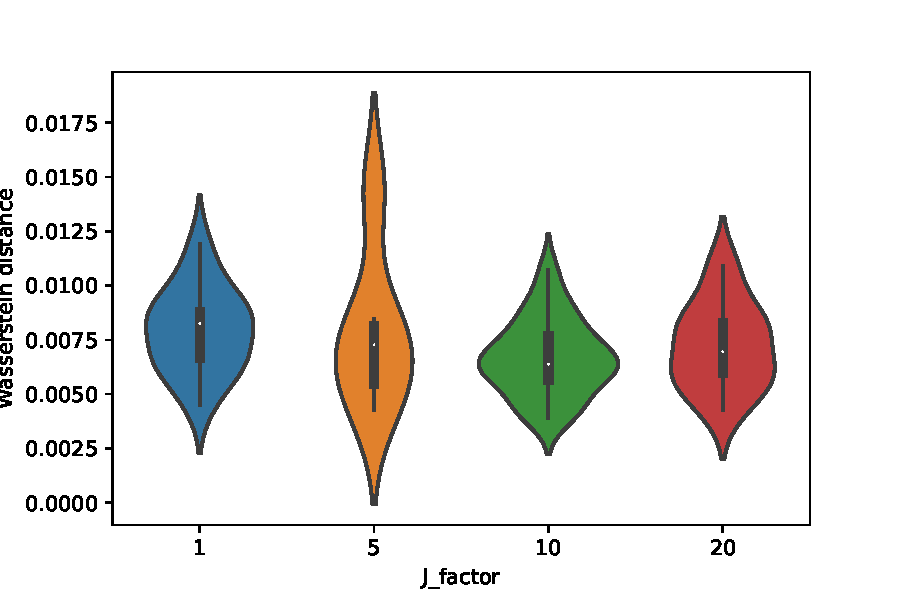
\includegraphics[scale=1]{content/plots/halftime/wd_per_J_factor.pdf}
  \caption{…}
  \label{fig:hyperparameter:J_factor}
\end{figure}

\subsection{Number of epochs}
